% --------------------------------------------------------------------------------------
%                   LATEX TEMPLATE FOR DISSERTATION (HONS)
% --------------------------------------------------------------------------------------
\documentclass[11pt]{book}

\usepackage{amsfonts, amsmath, amssymb}  
\usepackage{times}

%\usepackage[backref=page,pagebackref=true,linkcolor = blue,citecolor = red]{hyperref}
%\usepackage[backref=page]{backref}

\usepackage{graphicx}
\DeclareGraphicsExtensions{.pdf,.png,.jpg}

\setlength{\oddsidemargin}{1.5cm}
\setlength{\evensidemargin}{0cm}
\setlength{\topmargin}{1mm}
\setlength{\headheight}{1.36cm}
\setlength{\headsep}{1.00cm}
%\setlength{\textheight}{20.84cm}
\setlength{\textheight}{19cm}
\setlength{\textwidth}{14.5cm}
\setlength{\marginparsep}{1mm}
\setlength{\marginparwidth}{3cm}
\setlength{\footskip}{2.36cm}


\begin{document}
\pagestyle{empty}

%: ----------------------------------------------------------------------
%:                  TITLE PAGE: name, degree,..
% ----------------------------------------------------------------------

\begin{center}

\vspace{1cm}

%%% Type the thesis title below%%%%%%%%%%%%%%%%
{\Huge         Hadoop Map/Reduce R package Enhancement}

\vspace{25mm} 


\includegraphics[width=3.5cm]{logo}

 \vspace{35mm}

%%%%%Type Your Name Below%%%%%%%%%%%%
{\Large       Noah Zhang}

	\vspace{1ex}

Department of Statistics

The University of Auckland

	\vspace{5ex}

 %%%%%Typing Your Supervisors Name Below%%%%%%%%%%%%
Supervisor:             Simon Urbanek

	\vspace{30mm}

A dissertation submitted in partial fulfillment of the requirements for the degree of BSc(Hons) in Statistics, The University of Auckland, 2020.

\end{center}

\newpage


%: --------------------------------------------------------------
%:                  FRONT MATTER:  abstract,..
% --------------------------------------------------------------
\chapter*{Abstract}       
\setcounter{page}{1}
\pagestyle{headings}
% \pagenumbering{roman}

\addcontentsline{toc}{chapter}{Abstract}


 Put your abstract  here.  The abstract should contain a brief summary of the aim, methodologies, 
finding and conclusions of the dissertation.  The abstract should normally be fewer than 350 words.


Big data is concern massive amount, complex, growing data set from multiple autonomous sources. It has to deal with large
and complex dataset that can be structured, semi-structured or unstructured and will typically not fit into memory to be processed.
MapReduce is a programming model for processing large datasets distributed on a large clusters.A rapid growth of data in recent time,
Industries and academia required an intelligent data analysis tool that would be helpful to satisfy the need to analysis a large amount of
data. MapReduce framework is basically designed to compute data demanding applications to support effective decision making. Since
its introduction, remarkable research efforts have been put to make it more familiar to the users subsequently utilized to support the
execution of enormous data intensive applications. This survey paper highlights and investigates various applications using recent
MapReduce models.





%: --------------------------------------------------------------
%:                  END:  abstract
% --------------------------------------------------------------


%: ----------------------- contents ------------------------
\setcounter{secnumdepth}{3} % organisational level that receives a numbers
\setcounter{tocdepth}{3}    % print table of contents for level 3
\tableofcontents            % print the table of contents
% levels are: 0 - chapter, 1 - section, 2 - subsection, 3 - subsection

%: --------------------------------------------------------------
%:                  MAIN DOCUMENT SECTION
% --------------------------------------------------------------
	
\chapter{Introduction}%    \chapter{}  = level 1, top level

A thesis should always have an introduction.  The purpose is to describe the general subject area, state the research problem of interest, outline the main results of the thesis, and put the results in context with the wider subject area and its applications.

The main body of the text must be divided into a logical scheme which  is followed consistently throughout the work.  
 It usually starts with an introduction chapter  and ends with  a conclusion chapter. See, for example, the table of contents on page 3. 

There is strict  35-page limit  for an applied mathematics dissertation,  including  the references  but excluding  appendices. 

\section{Concept of Big Data}

Big data concerns huge amounts, complex and diverse sets of information that is growing at ever-increasing rates. The size of the data suggest that we will need to deviate from the traditional processing methodologies and to adapt an inexpensive and efficient way through distributed/parallel computing.\\

Today, we can find upwards of 800 million webpages providing documentation on big data. Enthusiasts believe that Big Data is the next big thing after Cloud [1]. 

\subsection{Characteristics of Big Data}

The concept of big data is generally vague without a formal definition, however the general consensus is that there are specific attributes that define big data The four characteristics of big data are Volume, Velocity, Variety and Veracity [2]. 

\begin{center}
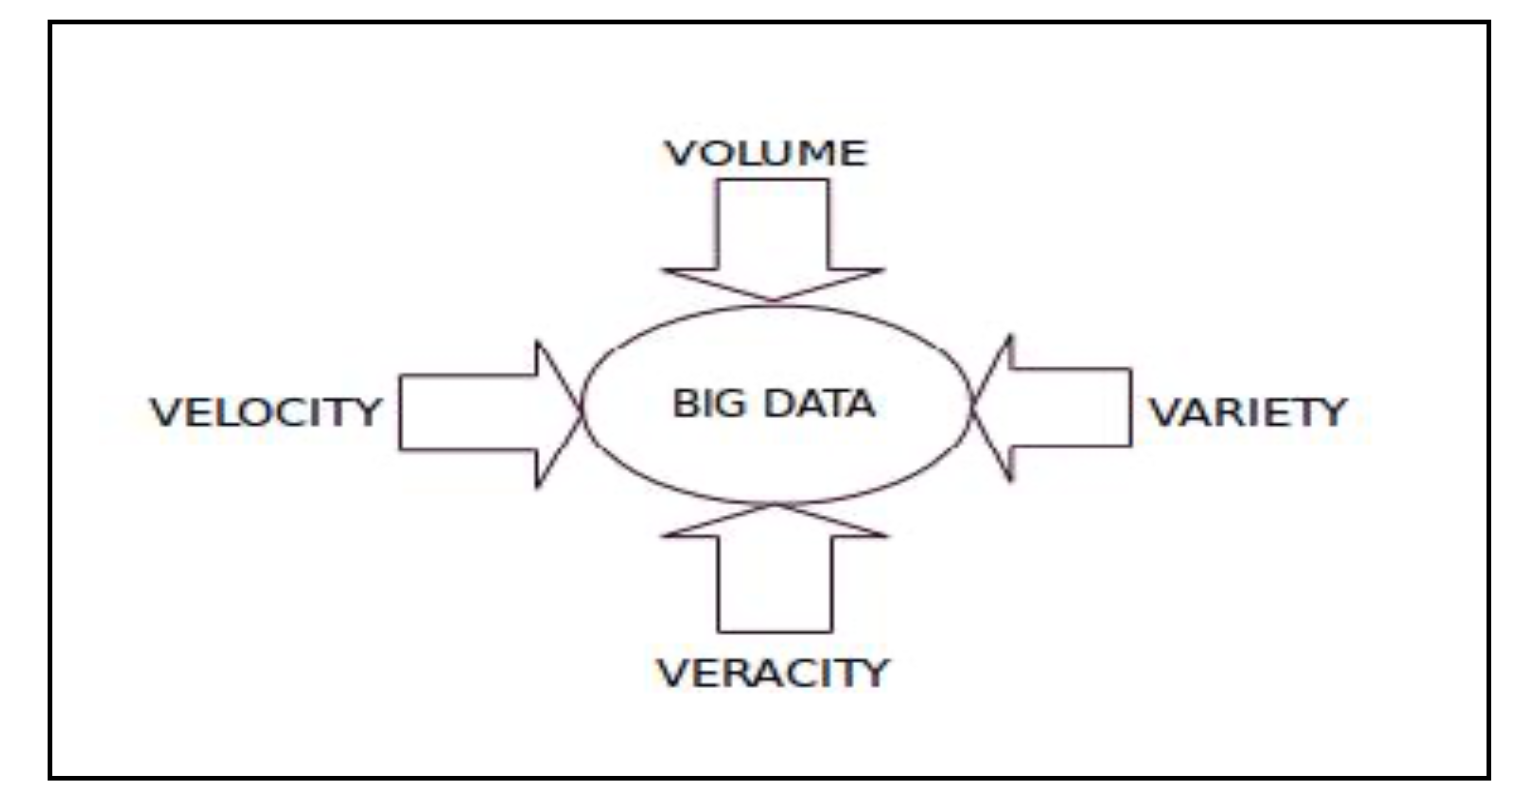
\includegraphics[width=10cm]{4vbd}\\
\end{center}

The main characteristic that makes data “big” is its sheer volume. According to estimates by IBM, we can expect at least 40 Zettabytes (43 Trillion Gigabytes) of data to be created in 2020 [3]. The volume of data sets being processed and analysed has reached sizes larger than terabytes and even petabytes. This suggests that data sets these days are becoming too large to process within a single desktop machine/processor. \\

Velocity is the speed at which data is generated. High velocity data is generated with such a pace that it may require certain distributed processing techniques. Good examples of high velocity data includes social media posts.\\

Variety is the source of the data which can be found in different forms such as text, numerical, images, audio and video records. The variety in the data will require distinct processing capabilities or algorithms to handle different formats. \\

Veracity is the quality of the data. Information may be volatile or incomplete seen in low veracity data sets containing a high percentage of meaningless data referred to as noise. On the other hand, high veracity data hold records that are valuable to analyse and contribute in a meaningful way to the overall results.

\subsection{Structure of Big Data} 

Big data can be categorised as structured or unstructured.\\
 
Structured data is usually stored and managed in relational databases with predefined data models. Examples of relational database applications with structured data include customer information, sales transactions, airline reservations systems, and billing systems. This type of structured data within relational databases can be accessed using Structured Query language (SQL).\\
 
Unstructured data, in contrast, has its internal structure but it is not structured through pre-defined data models or schema. As it may comes in many different formats, it cannot be stored in relational databases which also becomes a real challenge for systems to process and analyse. The unstructured data may be stored within non-relational databases like NoSQL.

\section{The Hadoop Framework}

At present, with data being generated at an exponential rate, there is the need to deploy data intensive application and storage clusters in order to keep up with the amount of data. To handle such problem, Google introduced the MapReduce model for distributed computing based on Java. This system is implemented through Apache Hadoop which is an open source software framework. This framework offers reliable, scalable, parallel and distributed computing scaling up from a single server to a network of multiple computers[4]. Apache Hadoop was developed with the purpose of having a data store that allow organisations to leverage big data analytics with cost efficiency in mind.\\

%There are two main components of Hadoop: Storage and Processing

\subsection{Hadoop Architecture}

Hadoop follows a master/slave architecture design for data storage and distributed data processing using HDFS and MapReduce respectively. The master node for data storage is NameNode while the master node for parallel processing is the Job Tracker. The slave nodes are comprised of other machines in the Hadoop cluster which stores the data and performs the computations. Each slave node have a DataNode and a TaskTracker that synchronises the process respectively. \\

 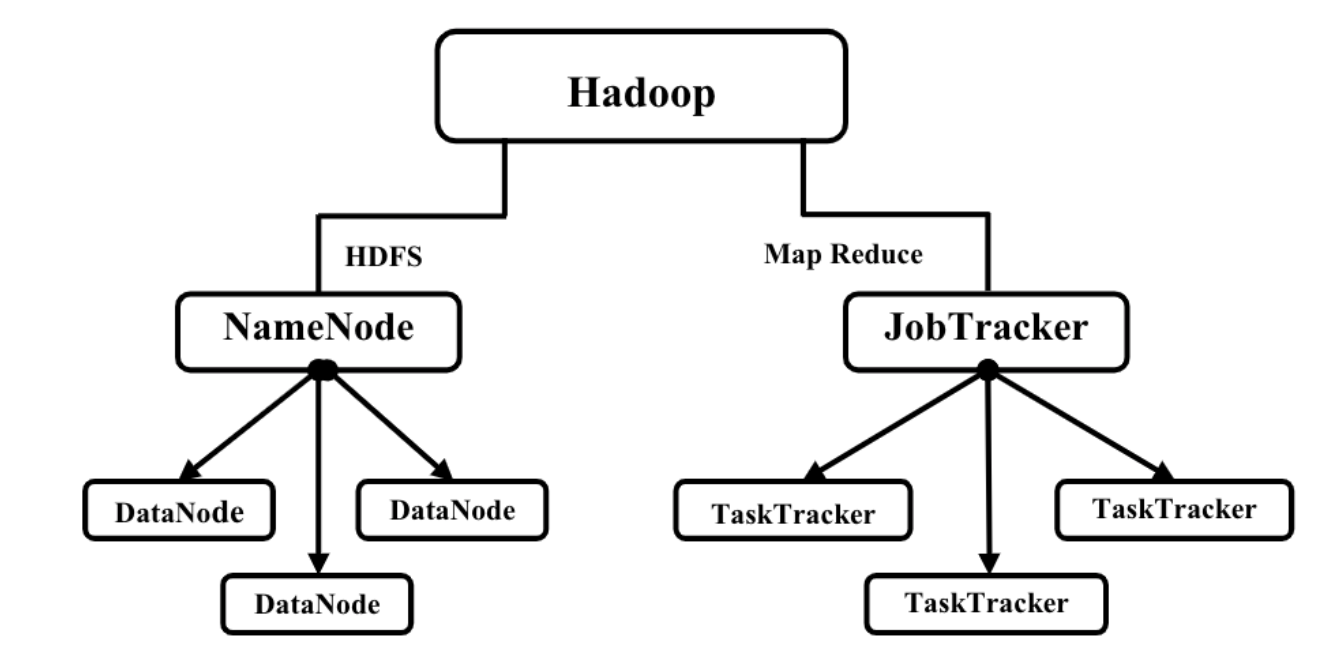
\includegraphics[width=10cm]{hadoop}\\

The Hadoop system can be set up via cloud or locally. The cluster we will be running is a set up of 8 virtual machines.

\subsection{Storage - HDFS}

The storage component of the Hadoop architecture is known as the Hadoop Distributed File System (HDFS). The NameNode runs on the master node and manages metadata about the file system in a file named fsimage. This metadata is cached in main memory to provide faster access to the clients on read/write requests. The NameNode controls also manages the slaves by splitting files into chunks (default 64 megabytes) and distributing them across each DataNode in the cluster. The DataNodes are primary storage elements of HDFS where chunks of data are stored and replicated according to the instructions from the NameNode. Secondary NameNode is to periodically read the file system, log changes and applying them to the fsimage file. This will enable the NameNode to boot faster.

The main advantages of HDFS is data locality and fault tolerance. Data locality allow the nodes to manipulate the data they have access to which results in faster and more efficient processing while handling faults through the process of replicating files across each slave node[4].\\

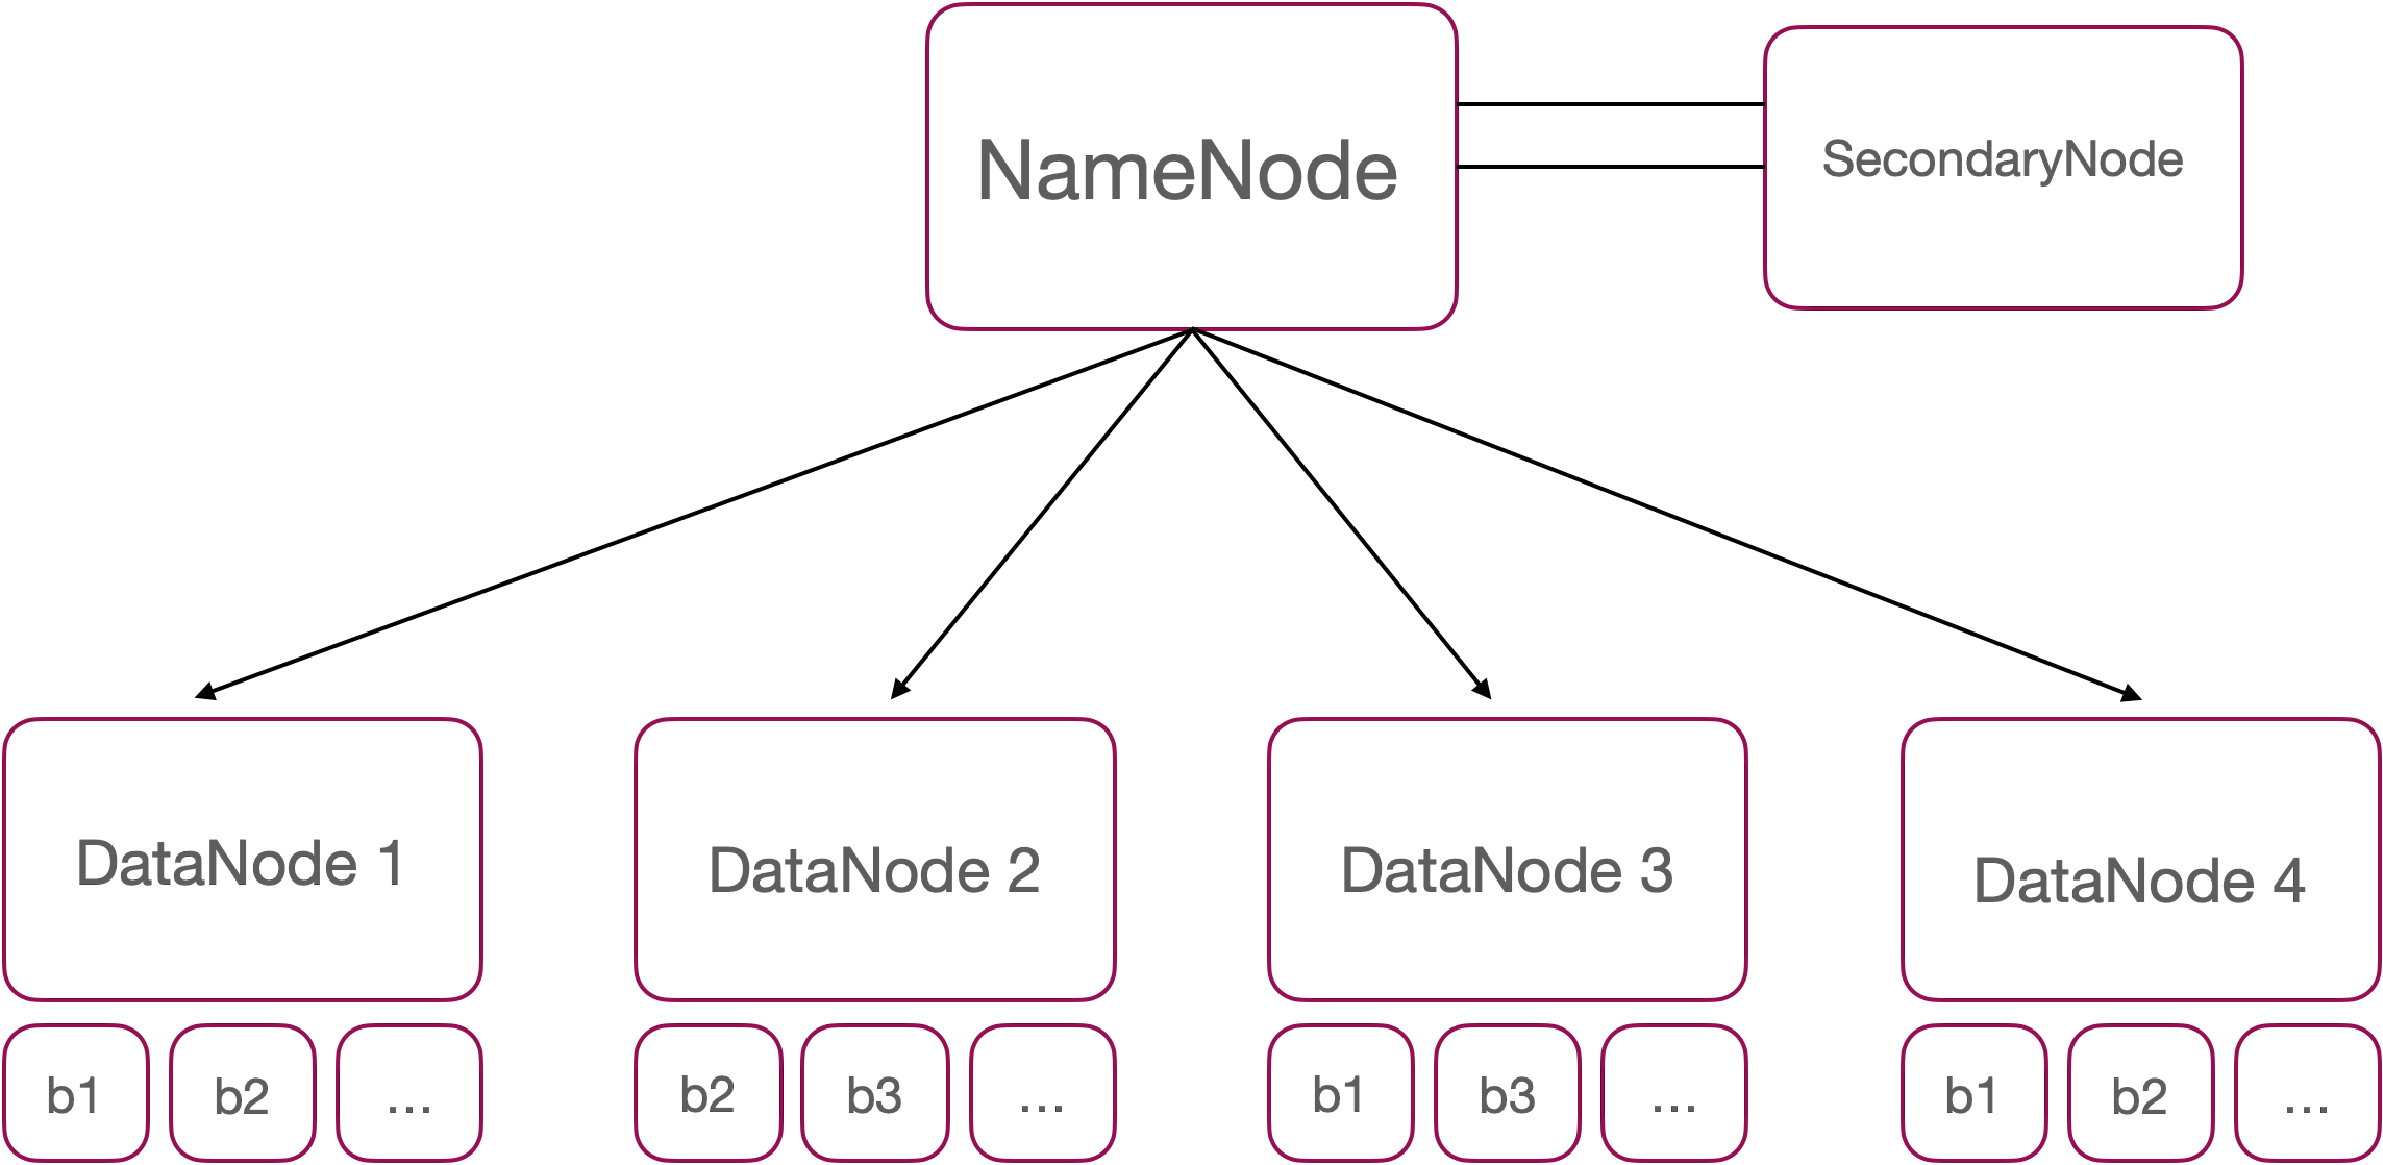
\includegraphics[width=8cm]{hdfs}

\subsection{Processing - MapReduce}

















\subsection{Equations}
The main strength of LaTex is  mathematical typesetting.  

There is a huge amount of information about LaTex on the internet.
A helpful short manual, also included in this folder, is the file
\verb+latex_intro.pdf+
This document gives a lot of sample LaTex commands.  
The file \verb+latex-howto.tex+ in this folder also contains examples of many latex commands.




We first show  some simple examples of 
mathematical formulae using latex typesetting.





\section{References}
1. BIG DATA: Challenges and opportunities, Infosys Lab Briefings,
Vol 11 No 1, 2013. \\

2. Big Data And Hadoop: A Review Paper, Rahul Beakta, 2015 \\

 3. IBM Big Data analytics HUB,
www.ibmbigdatahub.com/infographic/four-vs-big-data

4. Hadoop, MapReduce and HDFS: A Developers Perspective, 
Mohd Rehan Ghazi, Durgaprasad Gangodkar, 2015

5. MapReduce: Simplified Data Processing on Large Clusters, 
Jeffrey Dean and Sanjay Ghemawat


\end{document}
